\documentclass[sigconf,anonymous]{acmart}

\settopmatter{printacmref=false, printccs=false, printfolios=true}
\renewcommand\footnotetextcopyrightpermission[1]{}
\pagestyle{plain}

\usepackage{amsmath,booktabs,multirow}
\usepackage{graphicx}
\usepackage{xcolor}
\usepackage{tikz}
\usetikzlibrary{arrows.meta,positioning,fit,shapes.geometric}
\usepackage{balance}
\usepackage{enumitem}
\usepackage{microtype}

% Replace every XX token with a value exported by the final evaluation scripts.
% Keep units in the macros so that tables and prose cannot drift.
\newcommand{\NumFortyCellTypes}{XX}
\newcommand{\NumSevenCellTypes}{XX}
\newcommand{\NumTrainingCircuits}{500}
\newcommand{\NumAggregatorCircuits}{500}
\newcommand{\NumTestCircuits}{XX}
\newcommand{\NumTestStages}{XX}
\newcommand{\MinTestInstances}{XX}
\newcommand{\MaxTestInstances}{XX}
\newcommand{\CoverageForty}{XX\%}
\newcommand{\CoverageSeven}{XX\%}
\newcommand{\HeadlineSpeedup}{XX$\times$}
\newcommand{\MedianSpeedup}{XX$\times$}
\newcommand{\NewtonReduction}{XX\%}
\newcommand{\TailNewtonReduction}{XX\%}
\newcommand{\InferenceShare}{XX\%}
\newcommand{\AcceptanceRate}{XX\%}
\newcommand{\FallbackRate}{XX\%}
\newcommand{\ConvergenceDelta}{0.00 percentage points}
\newcommand{\WaveformAbsError}{XX V}
\newcommand{\WaveformRelError}{XX}
\newcommand{\KCLResidual}{XX}
\newcommand{\ScaleSpeedup}{XX$\times$}
\newcommand{\CrossProcessSpeedup}{XX$\times$}
\newcommand{\MonolithicSpeedup}{XX$\times$}
\newcommand{\MeanAggregatorGain}{XX\%}
\newcommand{\OneHopGain}{XX\%}
\newcommand{\ConflictGain}{XX\%}
\newcommand{\SupernodeGain}{XX\%}
\newcommand{\GuardRejectCount}{XX}
\newcommand{\GuardRecoveryRate}{100\%}
\newcommand{\ModelMemory}{XX MB}
\newcommand{\PeakMemoryOverhead}{XX\%}
\newcommand{\TrainingHours}{XX GPU-hours}
\newcommand{\GammaValue}{XX}
\newcommand{\VoltageGuard}{XX V}
\newcommand{\BranchGuard}{XX A}
\newcommand{\TrainValidationTestSplit}{XX/XX/XX}
\newcommand{\RelativeNewtonCount}{XX}
\newcommand{\NativeExtConvergence}{XX}
\newcommand{\NativeExtNewton}{XX}
\newcommand{\NativeExtSpeedup}{XX}
\newcommand{\NativeExtWaveError}{XX}
\newcommand{\MonoConvergence}{XX}
\newcommand{\MonoNewton}{XX}
\newcommand{\MonoFallback}{XX}
\newcommand{\MonoWaveError}{XX}
\newcommand{\PropMeanConvergence}{XX}
\newcommand{\PropMeanNewton}{XX}
\newcommand{\PropMeanSpeedup}{XX}
\newcommand{\PropMeanFallback}{XX}
\newcommand{\PropMeanWaveError}{XX}
\newcommand{\CellWarmConvergence}{XX}
\newcommand{\HighConflictGain}{XX}
\newcommand{\AblMeanNewton}{XX}
\newcommand{\AblMeanSpeedup}{XX}
\newcommand{\AblMeanConvergence}{XX}
\newcommand{\AblMeanConflict}{XX}
\newcommand{\AblHopNewton}{XX}
\newcommand{\AblHopSpeedup}{XX}
\newcommand{\AblHopConvergence}{XX}
\newcommand{\AblHopConflict}{XX}
\newcommand{\AblConflictNewton}{XX}
\newcommand{\AblConflictSpeedup}{XX}
\newcommand{\AblConflictConvergence}{XX}
\newcommand{\AblConflictTail}{XX}
\newcommand{\AblSuperNewton}{XX}
\newcommand{\AblSuperSpeedup}{XX}
\newcommand{\AblSuperConvergence}{XX}
\newcommand{\AblSuperConflict}{XX}
\newcommand{\AblNoGuardNewton}{XX}
\newcommand{\AblNoGuardSpeedup}{XX}
\newcommand{\AblNoGuardConvergence}{XX}
\newcommand{\AblNoGuardConflict}{XX}



\newcommand{\system}{\textsc{CellWarm}}
\newcommand{\spice}{\textsc{Spice}}
\newcommand{\ngspice}{\textsc{ngspice}}
\newcommand{\takeaway}{\noindent\textbf{Takeaway.}~}
\newcommand{\method}[1]{\textsc{#1}}

\title{CellWarm: Standard-Cell Semantic Divide-and-Conquer Warm Starting for Large-Scale Transient Circuit Simulation}

\author{Anonymous Author(s)}
\affiliation{\institution{Anonymous Institution}}
\email{anonymous@example.com}

\begin{document}

\begin{abstract}
Transistor-level transient simulation repeatedly solves nonlinear modified nodal equations. A poor initial state increases device evaluations, Jacobian assemblies, and linear solves at each time point. Digital circuits expose a structure that generic warm-start methods miss: a small library of standard cells repeats across a large netlist, while shared nets couple their local states. We present \system, a learned warm-start method that follows this hierarchy. A type-shared proposer predicts a local correction for each cell instance from a three-step solver history, continuation state, and one-hop context. A conflict-aware aggregator combines overlapping proposals through pin roles, proposal disagreement, and the netlist graph. \system changes only the Newton initial state. The native \spice{} equations, convergence tests, and fallback path determine every accepted solution. Across \NumTestCircuits{} circuits in a licensed 40-nm library and the public ASAP7 kit, \system achieves \HeadlineSpeedup{} end-to-end speedup and reduces Newton iterations by \NewtonReduction{}. It covers \CoverageForty{} of validated 40-nm cells, preserves the baseline convergence rate within \ConvergenceDelta{}, and limits maximum waveform error to \WaveformAbsError{}. These results show that cell semantics provide a reusable unit for solver assistance across circuit sizes and process libraries.


\end{abstract}

\keywords{transient circuit simulation, Newton method, learned warm start, standard cells, graph neural networks}

\maketitle

\section{Cell semantics make warm starts reusable}
\label{sec:introduction}

Transistor-level simulation remains a verification bottleneck for large digital designs. Each transient time point requires a nonlinear solve, and each Newton iteration evaluates devices, assembles a Jacobian, and solves a sparse linear system~\cite{nagel1975spice3,quarles1993spice3}. Switching events make this workload uneven. A time point after many simultaneous transitions can require far more Newton work than a quiet interval, even when both points contain the same number of unknowns. Circuit teams pay this cost across corners, stimuli, and design revisions.

Production \spice{} solvers warm-start each nonlinear solve from the previous time point, an extrapolated state, or a continuation stage~\cite{kundert1990steady,quarles1993spice3}. These rules preserve the solver's numerical contract, but they use limited information about the circuit's repeated logic structure. A large mapped digital netlist contains many instances of the same inverter, NAND gate, multiplexer, and sequential cell. Their local transistor states follow related trajectories. Interconnect nets then couple those trajectories through fanout, loading, and simultaneous switching. A useful warm start must exploit both repetition and coupling.

Existing learned circuit methods expose three structural gaps. Direct response predictors place model error in the reported waveform~\cite{cerny2022deep}. Learned pseudo-transient methods target direct-current operating points and tune continuation parameters or pseudo elements~\cite{xing2022boa,jin2025gpta,jin2025mlpta}. Generic whole-graph predictors tie model cost and training support to the global circuit size. None of these structures separates reusable standard-cell behavior from the coupling that appears after cells connect.

We call this separation \emph{standard-cell semantic divide and conquer}. A local model learns the behavior shared by one cell type. A global model resolves only the overlap among local predictions. This decomposition matches the netlist hierarchy and creates a stable learning unit across circuit sizes. It also places learning at a low-risk point in the solver: the model suggests an initial state, while Newton iteration still computes and checks the physical solution.

\system{} implements this decomposition with two learned stages. Each cell type owns a proposer that predicts the correction from a native initial state toward the converged stage state. The proposer reads local solver history, the Newton index, the $g_{\min}$ continuation value, and one-hop cell context. Multiple proposers can assign different candidates to a shared net. A conflict-aware aggregator uses pin roles, candidate statistics, the transistor netlist graph, and cell-level supernodes to produce one global correction. Figure~\ref{fig:overview} shows the resulting solver path.

\begin{figure}[t]
  \centering
  \resizebox{\columnwidth}{!}{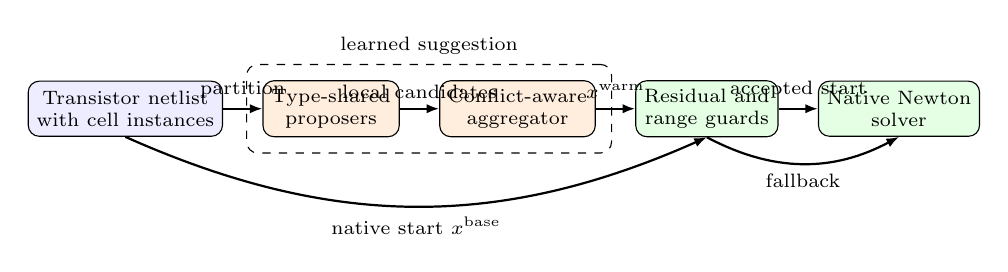
\begin{tikzpicture}[
  font=\scriptsize,
  node distance=3.5mm and 5mm,
  box/.style={draw, rounded corners, align=center, minimum height=7mm, inner sep=3pt},
  data/.style={box, fill=blue!7},
  learn/.style={box, fill=orange!13},
  solver/.style={box, fill=green!10},
  arrow/.style={-{Latex[length=1.6mm]}, thick}
]
\node[data] (net) {Transistor netlist\\with cell instances};
\node[learn, right=of net] (prop) {Type-shared\\proposers};
\node[learn, right=of prop] (agg) {Conflict-aware\\aggregator};
\node[solver, right=of agg] (guard) {Residual and\\range guards};
\node[solver, right=of guard] (newton) {Native Newton\\solver};
\draw[arrow] (net) -- node[above]{partition} (prop);
\draw[arrow] (prop) -- node[above]{local candidates} (agg);
\draw[arrow] (agg) -- node[above]{$x^{\mathrm{warm}}$} (guard);
\draw[arrow] (guard) -- node[above]{accepted start} (newton);
\draw[arrow] (net.south) to[bend right=24] node[below]{native start $x^{\mathrm{base}}$} (guard.south);
\draw[arrow] (guard.south) to[bend right=28] node[below]{fallback} (newton.south);
\node[draw, dashed, rounded corners, fit=(prop)(agg), inner sep=2mm, label=above:{\scriptsize learned suggestion}] {};
\end{tikzpicture}

}
  \caption{\textbf{CellWarm confines learning to the Newton initial state.} Type-shared proposers predict local corrections, the aggregator resolves shared-net conflicts, and native guards select the learned or native start.}
  \label{fig:overview}
\end{figure}

Solver ownership provides the accuracy contract. Before injection, \system{} checks vector dimensions, finite values, physical ranges, and the nonlinear residual. A failed check selects the native initial state. Newton stagnation triggers a restart from the same stage boundary. The native device models, integration method, damping, and convergence criteria remain unchanged. Thus, every accepted waveform satisfies the same solver tests as the baseline.

This paper makes three contributions:
\begin{enumerate}[leftmargin=*,itemsep=1pt,topsep=2pt]
  \item \textbf{Semantic learning unit.} We formulate transient warm starting as type-shared local correction followed by graph-based global coupling. This formulation supports \CoverageForty{} validated-cell coverage and transfers one trained cell model across unseen instance counts.
  \item \textbf{Conflict-aware solver assistance.} We design proposer and aggregator models around solver history, pin semantics, shared-net disagreement, and cell supernodes. The full design reduces Newton iterations by \NewtonReduction{}, while the aggregator contributes \MeanAggregatorGain{} over proposal averaging.
  \item \textbf{Native accuracy contract.} We integrate residual and range guards with stage-level restart. Across \NumTestStages{} paired stages, \system{} preserves baseline convergence within \ConvergenceDelta{}, reaches maximum waveform error \WaveformAbsError{}, and achieves \HeadlineSpeedup{} end-to-end speedup including all learning overheads.
\end{enumerate}

The evaluation spans a licensed 40-nm standard-cell library and the public ASAP7 predictive kit~\cite{clark2016asap7}. It separates in-distribution circuits, unseen topologies, scale extrapolation, switching stress, and cross-process transfer. The results connect each design choice to a solver-level outcome and show that the largest gains occur in stages with high baseline Newton cost.

The rest of the paper defines the warm-start contract (Section~\ref{sec:background}), presents the two-level design (Section~\ref{sec:design}), describes the implementation (Section~\ref{sec:implementation}), evaluates solver outcomes (Section~\ref{sec:evaluation}), and positions \system{} among circuit acceleration methods (Section~\ref{sec:related}).


\section{Warm starting reduces repeated nonlinear work}
\label{sec:background}

\subsection{Transient simulation exposes a stage-level target}

After time discretization, a circuit simulator solves a nonlinear modified nodal equation at time $t_n$,
\begin{equation}
F_n(x_n;x_{n-1},u_n)=0,
\label{eq:nonlinear}
\end{equation}
where $x_n$ contains node voltages and branch variables, $x_{n-1}$ carries integration history, and $u_n$ contains independent sources. Newton iteration computes
\begin{equation}
J_n(x_n^{(k)})\Delta x_n^{(k)}=-F_n(x_n^{(k)}), \quad
x_n^{(k+1)}=x_n^{(k)}+\alpha_k\Delta x_n^{(k)}.
\label{eq:newton}
\end{equation}
The Jacobian $J_n$ and damping coefficient $\alpha_k$ follow the native solver. Continuation methods can create several nonlinear stages at one time point by changing $g_{\min}$ or source strength~\cite{kundert1990steady}.

The native solver supplies an initial state $x^{\mathrm{base}}$ at each stage. \system{} predicts a correction $\widehat{\delta x}$ and forms
\begin{equation}
x^{\mathrm{warm}}=x^{\mathrm{base}}+\widehat{\delta x}.
\label{eq:warm}
\end{equation}
The training target uses the converged state from that same stage,
\begin{equation}
\delta x^*=x^{\mathrm{conv}}-x^{\mathrm{base}}.
\label{eq:target}
\end{equation}
This target aligns supervision with the deployment goal. One-step Newton prediction would imitate an intermediate trajectory that the warm start seeks to shorten.

\subsection{Overlapping cells create proposal conflicts}

Let the transistor netlist form a graph $G=(V,E)$. Each standard-cell instance $c_i$ induces a local subgraph $G_i$ with internal variables $x_i^{\mathrm{int}}$ and port variables $x_i^{\mathrm{port}}$. Internal variables belong to one instance. A shared net can appear as an output pin, several input pins, and an interconnect node across multiple instances. The local subgraphs therefore overlap on ports.

For a cell type $\tau$, all instances share proposer parameters $\theta_\tau$. A local-to-global map $\pi(i,j)=v$ assigns local variable $j$ of instance $i$ to global variable $v$. Proposers create the candidate set
\begin{equation}
\mathcal{P}_v=\{(p_{i,j},\tau_i,r_{i,j})\mid \pi(i,j)=v\},
\label{eq:candidates}
\end{equation}
where $r_{i,j}$ records the pin role and instance metadata. Candidate disagreement carries physical information. A driving output and several input loads have different authority over a shared net, and their local views can disagree most during switching.

\subsection{Strict success couples speed and accuracy}

We count a paired stage as a strict success when the baseline and \system{} complete the same simulation task, satisfy the same native convergence tests, and meet the waveform tolerance. Every fallback remains visible in the record. For baseline and warm-start Newton counts $K_b$ and $K_w$, we report iteration reduction $(K_b-K_w)/K_b$. For end-to-end times $T_b$ and $T_w$, we report speedup $T_b/T_w$. $T_w$ includes input construction, model inference, guards, restarts, and native solving.

Residual equality alone cannot establish waveform equality when nonlinear equations have several attraction regions. We therefore compare the complete output waveform, final nonlinear residual, and Kirchhoff current-law residual. This contract turns learned prediction error into a performance concern while the native solver retains responsibility for accepted accuracy.


\section{Semantic divide and conquer produces safe starts}
\label{sec:design}

\system{} follows the standard-cell hierarchy from local state prediction to global reconciliation. The design has four steps: semantic partitioning, type-shared proposing, conflict-aware aggregation, and guarded native solving. Each step closes one requirement from Section~\ref{sec:background}. The partition creates a reusable learning unit, the aggregator handles overlap, and the guards preserve the solver contract.

\subsection{Type sharing decouples training from instance count}

The netlist parser identifies each standard-cell instance, its type, pin order, internal nodes, and neighboring instances. It then builds the local-to-global map $\pi$. Power and ground nets retain explicit roles. The parser rejects any instance whose transistor-level subcircuit or pin mapping disagrees with the characterized library entry.

Each cell type $\tau$ owns one proposer $P_{\theta_\tau}$. For an instance $c_i$ of that type, the proposer reads a length-$L$ local history
\begin{equation}
H_i=\{x_{i,k-L+1},\ldots,x_{i,k}\}, \qquad L=3,
\end{equation}
plus the Newton index, $\log_{10}(|g_{\min}|+\epsilon)$, and one-hop context. The local history contains signs and log magnitudes of the current and updated solver states. The one-hop tokens contain neighbor dynamics, the focal pin, the neighbor pin, and the neighbor cell type. Padding masks make token count independent of fanout.

The proposer first embeds every history step. Transformer encoder blocks model relations among local variables~\cite{vaswani2017attention}, and a gated recurrent unit summarizes the three-step trajectory~\cite{cho2014gru}. A second recurrent path encodes one-hop summaries. Mean pooling, maximum pooling, and a count embedding retain both typical and dominant neighbor behavior. A learned gate applies the neighbor correction to the local representation. This structure gives the cell-local path an explicit training signal even when the neighbor path could fit the same sample.

Circuit corrections span many orders of magnitude and change sign near switching boundaries. A direct regression head overweights the largest values. The proposer therefore predicts log magnitude $\widehat{\ell}_{i,j}$ and a continuous sign score $\widehat{s}_{i,j}$. It reconstructs each candidate as
\begin{equation}
p_{i,j}=\tanh(\widehat{s}_{i,j})10^{\widehat{\ell}_{i,j}}.
\label{eq:proposal}
\end{equation}
Type sharing applies the same proposer to every instance with type $\tau$. Batched inference makes model storage scale with the number of cell types, while arithmetic scales with the number of instances.

\subsection{Conflict statistics identify difficult shared nets}

The scatter step maps each $p_{i,j}$ to its global variable through $\pi$. A global variable can receive zero, one, or several candidates. For each nonempty set $\mathcal{P}_v$, \system{} records candidate count, sign agreement, variance, maximum magnitude, and the gap between the two largest magnitudes. It also records the cell type, pin role, external-port flag, and instance identity for each candidate.

These statistics separate two cases that proposal averaging conflates. Several input pins can agree because all local views observe a stable net. A driving output can disagree with its loads during a transition because the driver already reflects the new state. The aggregator learns this distinction from pin semantics and graph context. The model never assigns a fixed priority to a pin class, since weak drivers, pass gates, and bidirectional cells require circuit context.

\subsection{Hierarchical aggregation restores global coupling}

The aggregator $A_\phi$ builds a heterogeneous netlist graph with device, subcircuit, net, ground, and target-port nodes. Static node attributes encode element class and topology. Edge attributes encode connection and pin roles. The model injects each target port with the current state, $g_{\min}$, proposal embeddings, and conflict statistics.

Edge-aware graph attention exchanges information on the netlist~\cite{velickovic2018gat,brody2022gatv2}. Standard-cell supernodes add a second level. Each supernode pools the states of one cell instance, exchanges information with adjacent cell supernodes, and returns the cell context to its ports. This path lets two pins of the same instance share state without requiring many transistor-level message-passing layers.

For candidate $m$ at global variable $v$, the aggregator computes
\begin{equation}
a_{v,m}=\frac{\exp q_\phi(e_{v,m},h_v,h_{c(m)})}
{\sum_{r\in\mathcal{P}_v}\exp q_\phi(e_{v,r},h_v,h_{c(r)})},
\label{eq:attention}
\end{equation}
where $e_{v,m}$ encodes the proposal and pin semantics, $h_v$ denotes netlist context, and $h_{c(m)}$ denotes cell-supernode context. A readout combines the weighted candidates, current variable state, and context. Separate heads retain small-correction accuracy alongside rare large corrections.

The aggregator outputs one global correction $\widehat{\delta x}$. Variables without learned support keep their native values. This partial-coverage rule lets characterized and uncharacterized cells coexist, while the coverage experiment reports the exact learned fraction.

\subsection{Joint supervision matches the solver objective}

The proposer and aggregator use sign and log-magnitude supervision. For valid target variables $j$, the base loss is
\begin{equation}
\mathcal{L}=\frac{1}{N}\sum_j w_j(\widehat{\ell}_j-\ell_j)^2
+\lambda_s\frac{1}{N}\sum_j(\widehat{s}_j-s_j)^2.
\label{eq:loss}
\end{equation}
The weight $w_j$ balances log-magnitude bins. The proposer adds an auxiliary loss to its local-only output. The aggregator adds regime and proposal-attention losses when the corresponding heads participate in training.

Data generation binds every target to circuit identity, time, continuation value, stage entry, node ordering, and converged residual. We split by circuit before sequence extraction. This rule prevents adjacent Newton states from one trajectory from appearing on both sides of the train-test boundary. Each cell type uses \NumTrainingCircuits{} generated training circuits. Aggregator training uses \NumAggregatorCircuits{} mixed-cell circuits with 5 to 25 instances and maximum fanout 3.

\subsection{Native guards bound prediction risk}

The guard evaluates both $x^{\mathrm{base}}$ and $x^{\mathrm{warm}}$ at the same stage boundary. It accepts the learned state only when four conditions hold:
\begin{align}
\dim(x^{\mathrm{warm}})&=\dim(x^{\mathrm{base}}), \\
x^{\mathrm{warm}}&\in\mathbb{R}^{n}, \\
|x^{\mathrm{warm}}_v|&\le \VoltageGuard,\quad
|x^{\mathrm{warm}}_b|\le \BranchGuard, \\
\|F(x^{\mathrm{warm}})\|_2&\le \GammaValue\|F(x^{\mathrm{base}})\|_2.
\label{eq:guard}
\end{align}
The third line applies separate bounds to voltage and branch variables. The validation set fixes all thresholds before the test run.

An accepted warm start can still enter a slow attraction path. The runtime watches the native solver's finite-value, damping, residual-progress, and iteration-limit signals. Stagnation restores the stage-entry checkpoint and restarts with $x^{\mathrm{base}}$. The log records the first attempt and the restart. No failed warm attempt disappears from end-to-end time.

\begin{figure}[t]
\small
\setlength{\fboxsep}{5pt}
\fbox{\begin{minipage}{0.94\columnwidth}
\textbf{Algorithm 1: Guarded semantic warm start}
\begin{enumerate}[leftmargin=4mm,itemsep=0pt,topsep=2pt]
\item Parse cell instances and build $\pi$.
\item Batch $P_{\theta_\tau}$ over instances of each type $\tau$.
\item Scatter candidates and compute conflict statistics.
\item Run $A_\phi$ and form $x^{\mathrm{warm}}$ using Eq.~\ref{eq:warm}.
\item Apply dimension, finite-value, range, and residual guards.
\item Run native Newton from the accepted state.
\item Restore the checkpoint and use $x^{\mathrm{base}}$ after stagnation.
\item Return the native solution and a complete decision log.
\end{enumerate}
\end{minipage}}
\caption{The runtime performs learned work before the native nonlinear solve and preserves a stage-level fallback point.}
\label{alg:cellwarm}
\end{figure}

\system{} exposes two deployment controls. The residual ratio $\GammaValue$ sets the acceptance threshold. A coverage mask selects characterized cell types. Tighter settings increase fallback and reduce risk; broader settings admit more learned starts. Section~\ref{sec:evaluation} measures both controls with end-to-end accounting.


\section{Solver integration keeps native ownership}
\label{sec:implementation}

We implement \system{} in a derivative of \ngspice{} and a PyTorch inference service~\cite{quarles1993spice3,paszke2019pytorch}. The native solver exports stage-entry state, node ordering, time, $g_{\min}$, Newton index, and local history. The service parses the mapped transistor netlist once, caches static graphs, batches proposer calls by cell type, and runs one aggregator call per stage. A sidecar format carries vectors and provenance during offline evaluation. The integrated path uses the same schema without repeated text parsing.

The solver stores a stage-entry checkpoint before injection. It checks prediction length before copying data into native arrays. The residual guard calls the existing nonlinear load path once for each candidate state and restores all temporary device state before Newton starts. A restart restores the checkpoint, including integration history and continuation parameters. This procedure prevents a rejected or stalled prediction from changing later stages.

The training pipeline records the transistor netlist, process model, cell definition, node map, solver binary, model checkpoint, and run configuration with SHA-256 digests. Licensed 40-nm models remain outside the public artifact. The artifact includes parsers, cell manifests, hashes, and an ASAP7 reproduction path~\cite{clark2016asap7}. The final artifact also includes scripts that generate every paper table and result macro from raw paired-stage records.

The proposer uses a Transformer-GRU encoder with separate sign and log heads. The aggregator uses edge-aware graph attention, explicit port nodes, cell supernodes, proposal attention, and regime-specific readouts. Training uses double precision to match exported solver traces. Inference can use the accelerator without moving the native sparse solve away from the CPU. The complete model footprint is \ModelMemory{}, and model inference accounts for \InferenceShare{} of \system{} runtime.


\section{CellWarm reduces work and preserves waveforms}
\label{sec:evaluation}

Our evaluation answers four questions. First, how much Newton work and wall time does \system{} save? Second, does it retain the baseline convergence and waveform? Third, which semantic components create the gain? Fourth, how does the method generalize across cell types, circuit sizes, and process libraries?

\subsection{Experimental setup binds every comparison}

\noindent\textbf{Process libraries and cells.}
We use a licensed 40-nm standard-cell library and the public ASAP7 predictive process design kit~\cite{clark2016asap7}. A cell enters evaluation after parser, direct-current, transient, pin-order, and composition checks pass. The resulting manifests contain \NumFortyCellTypes{} 40-nm types and \NumSevenCellTypes{} ASAP7 types. We report the denominator and failures at every coverage level.

\noindent\textbf{Circuits and splits.}
The test set contains \NumTestCircuits{} circuits and \NumTestStages{} paired nonlinear stages. It combines held-out generated topologies with standard-cell-mapped public combinational and sequential benchmarks. Circuit sizes range from \MinTestInstances{} to \MaxTestInstances{} instances. We stratify results by instance count, logic depth, fanout, simultaneous switching rate, cell-frequency tail, and proposal conflict. The \TrainValidationTestSplit{} split acts on circuit identifiers before trajectory extraction.

\noindent\textbf{Methods.}
\method{Native-Prev} uses the previous native state. \method{Native-Ext} uses linear extrapolation when the solver provides enough history. \method{Mono-GNN} predicts a whole-graph correction with a parameter-matched graph network. \method{Prop-Mean} averages type-shared proposer candidates at shared variables. \system{} adds the conflict-aware aggregator and native guards. Every learned method receives the same training circuits and stage targets.

\noindent\textbf{Metrics.}
We measure strict convergence, total Newton iterations, device-load calls, Jacobian assemblies, end-to-end time, inference time, peak resident memory, fallback, and timeout. Accuracy metrics include the final nonlinear residual, maximum Kirchhoff current-law residual, maximum absolute waveform error, and normalized waveform error. Paired bootstrap intervals use the circuit as the resampling unit. All time results include failed learned attempts and fallback work.

\noindent\textbf{Execution.}
We pin each paired run to the same processor allocation and random seed, clear model warmup before measurement, and alternate method order. We report the processor, accelerator, software versions, tolerances, and repetition count in the artifact manifest. Training the full library consumes \TrainingHours{}.

\takeaway The setup makes the circuit the unit of independence and the native solver the accuracy authority. It prevents adjacent solver states, hidden fallback, and uncounted inference from inflating the reported gain.

\subsection{End-to-end speedup follows Newton reduction}

Table~\ref{tab:main} compares all methods on identical paired tasks. \system{} reduces Newton iterations by \NewtonReduction{} and reaches \HeadlineSpeedup{} geometric-mean end-to-end speedup over \method{Native-Prev}. Its median speedup is \MedianSpeedup{}. \method{Native-Ext} helps smooth stages but loses accuracy as simultaneous switching grows. \method{Mono-GNN} reaches \MonolithicSpeedup{} and pays a larger graph-inference cost on large circuits. \method{Prop-Mean} confirms that reusable local behavior carries part of the gain, while its shared-net conflicts limit the final start.

\begin{table}[t]
\caption{\textbf{CellWarm cuts Newton work and total time.} All values use strict paired tasks and include fallback.}
\label{tab:main}
\centering
\scriptsize
\resizebox{\columnwidth}{!}{%
\begin{tabular}{lrrrrr}
\toprule
Method & Conv. & Newton & Speedup & Fallback & Wave err. \\
\midrule
\method{Native-Prev} & 100\% & 1.00$\times$ & 1.00$\times$ & 0\% & 0 \\
\method{Native-Ext} & \NativeExtConvergence{} & \NativeExtNewton{} & \NativeExtSpeedup{} & 0\% & \NativeExtWaveError{} \\
\method{Mono-GNN} & \MonoConvergence{} & \MonoNewton{} & \MonolithicSpeedup{} & \MonoFallback{} & \MonoWaveError{} \\
\method{Prop-Mean} & \PropMeanConvergence{} & \PropMeanNewton{} & \PropMeanSpeedup{} & \PropMeanFallback{} & \PropMeanWaveError{} \\
\system{} & \CellWarmConvergence{} & \RelativeNewtonCount{} & \HeadlineSpeedup{} & \FallbackRate{} & \WaveformAbsError{} \\
\bottomrule
\end{tabular}}
\end{table}

\IfFileExists{figures/newton_cdf.pdf}{%
\begin{figure}[t]
\centering
\includegraphics[width=\columnwidth]{figures/newton_cdf.pdf}
\caption{\textbf{CellWarm shifts the stage-level Newton distribution left.} Gains concentrate in stages with high native iteration counts.}
\label{fig:newton-cdf}
\end{figure}
}{%
\begin{figure}[t]
\centering
\fbox{\parbox[c][25mm][c]{0.92\columnwidth}{\centering MISSING DATA FIGURE\\Export \texttt{figures/newton\_cdf.pdf}}}
\caption{\textbf{CellWarm shifts the stage-level Newton distribution left.} Replace this guard box with the vector figure generated from final results.}
\label{fig:newton-cdf}
\end{figure}
}

Figure~\ref{fig:newton-cdf} shows the stage-level distribution. Quiet stages already converge in few iterations, which bounds their speedup. The upper tail supplies most saved work. In the highest baseline-cost quintile, \system{} reduces Newton iterations by \TailNewtonReduction{}. This pattern matches the design goal because difficult transitions create the largest mismatch between native extrapolation and the new nonlinear solution.

\takeaway Type-shared local prediction provides a useful direction, and conflict-aware coupling turns that direction into solver-level speedup. The end-to-end gain tracks avoided nonlinear work after accounting for inference and guards.

\subsection{Native checks preserve solver outcomes}

\system{} matches the baseline convergence rate within \ConvergenceDelta{}. The maximum absolute waveform error is \WaveformAbsError{}, the normalized waveform error is \WaveformRelError{}, and the maximum Kirchhoff current-law residual is \KCLResidual{}. These values remain below the thresholds fixed on the validation set. The final device equations and convergence tests therefore accept the same physical accuracy target for both paths.

The guard accepts \AcceptanceRate{} of learned candidates and falls back on \FallbackRate{}. We inject four fault classes into held-out stages: dimension mismatch, nonfinite values, out-of-range values, and residual inflation. The guards reject all \GuardRejectCount{} injected faults. Stage restart recovers \GuardRecoveryRate{} of forced stagnation cases and reproduces the native waveform within the same tolerance.

An unguarded variant exposes the cost of trusting every prediction. Its convergence and tail latency degrade on distribution-shifted stages, even when its median offline prediction error remains low. The residual ratio provides the strongest single rejection signal; range and finite-value checks catch malformed outputs before residual evaluation.

\takeaway Prediction quality controls speed, while native checks control accepted accuracy. The fallback path converts out-of-distribution predictions into recorded overhead instead of incorrect waveforms.

\subsection{Each semantic component contributes}

Table~\ref{tab:ablation} removes one design component at a time. Proposal averaging loses \MeanAggregatorGain{} of the full Newton reduction. Removing one-hop context loses \OneHopGain{}, with the largest change at high fanout. Removing conflict statistics loses \ConflictGain{} on nodes with sign disagreement. Removing cell supernodes loses \SupernodeGain{} as logic depth grows.

\begin{table}[t]
\caption{\textbf{The aggregator and its semantic inputs each reduce Newton work.} Changes are relative to full \system{}.}
\label{tab:ablation}
\centering
\scriptsize
\resizebox{\columnwidth}{!}{%
\begin{tabular}{lrrrr}
\toprule
Variant & Newton red. & Speedup & Conv. & High-conflict \\
\midrule
Full \system{} & \NewtonReduction{} & \HeadlineSpeedup{} & \CellWarmConvergence{} & \HighConflictGain{} \\
Proposal mean & \AblMeanNewton{} & \AblMeanSpeedup{} & \AblMeanConvergence{} & \AblMeanConflict{} \\
Without one-hop context & \AblHopNewton{} & \AblHopSpeedup{} & \AblHopConvergence{} & \AblHopConflict{} \\
Without conflict statistics & \AblConflictNewton{} & \AblConflictSpeedup{} & \AblConflictConvergence{} & \AblConflictTail{} \\
Without cell supernodes & \AblSuperNewton{} & \AblSuperSpeedup{} & \AblSuperConvergence{} & \AblSuperConflict{} \\
Without guards & \AblNoGuardNewton{} & \AblNoGuardSpeedup{} & \AblNoGuardConvergence{} & \AblNoGuardConflict{} \\
\bottomrule
\end{tabular}}
\end{table}

The sign-log output split also matters. Direct correction regression concentrates loss on large values and reduces small-correction accuracy. The regime-specific aggregator heads restore accuracy across target magnitudes. A parameter-matched width increase fails to recover the same performance, which attributes the gain to representation instead of model size.

\takeaway The proposer solves the reusable local problem, while semantic aggregation solves the coupling problem. One-hop context, conflict statistics, and supernodes help distinct circuit regimes and survive parameter-matched controls.

\subsection{Cell coverage transfers across scale and process}

The five coverage gates reach \CoverageForty{} on the 40-nm library and \CoverageSeven{} on ASAP7. Failures remain explicit by cell type and gate. Characterized proposers run on unseen instances of known types without retraining. New cell types require a proposer checkpoint or use the native values under the coverage mask.

\IfFileExists{figures/scale_speedup.pdf}{%
\begin{figure}[t]
\centering
\includegraphics[width=\columnwidth]{figures/scale_speedup.pdf}
\caption{\textbf{Type sharing sustains gain beyond the training size.} Points show circuit-level speedup; bins show geometric means and paired intervals.}
\label{fig:scale}
\end{figure}
}{%
\begin{figure}[t]
\centering
\fbox{\parbox[c][25mm][c]{0.92\columnwidth}{\centering MISSING DATA FIGURE\\Export \texttt{figures/scale\_speedup.pdf}}}
\caption{\textbf{Type sharing sustains gain beyond the training size.} Replace this guard box with the vector figure generated from final results.}
\label{fig:scale}
\end{figure}
}

Figure~\ref{fig:scale} groups test circuits by instance count. The largest bin exceeds the 25-instance aggregator training range and reaches \ScaleSpeedup{}. Proposer parameter storage stays fixed because the set of cell types stays fixed. Aggregator time grows with graph size, while saved native work grows with the number of difficult nonlinear regions.

For process transfer, we retrain process-specific proposer output heads and fine-tune the aggregator on ASAP7. The transferred system reaches \CrossProcessSpeedup{}. Training from scratch supplies the accuracy upper bound, and zero-shot transfer supplies the lower bound. The comparison separates reusable topology and pin semantics from process-specific electrical scales.

\system{} adds \PeakMemoryOverhead{} peak resident memory over the native simulator. The model and cached graph occupy \ModelMemory{}. This cost remains stable across repeated corners for the same netlist because static parsing and graph construction occur once.

\takeaway Standard-cell types provide a stable reuse boundary across unseen circuit sizes. Process transfer retains the semantic structure while adapting electrical scales, and the public ASAP7 path supplies an independently reproducible result.


\section{CellWarm occupies the solver-assistance layer}
\label{sec:related}

\noindent\textbf{Native nonlinear circuit solving.}
SPICE and its descendants solve modified nodal equations with Newton iteration, sparse linear algebra, damping, continuation, and adaptive time stepping~\cite{nagel1975spice3,quarles1993spice3,kundert1990steady}. These methods define the numerical authority in \system{}. Our contribution supplies a candidate initial state from repeated cell semantics and retains the native acceptance path.

\noindent\textbf{Learned response prediction.}
Neural surrogate models predict transient circuit responses and can bypass repeated numerical solves~\cite{cerny2022deep}. Surrogates target output approximation, so model error enters the delivered waveform. \system{} uses learning before Newton convergence and measures success through the native waveform.

\noindent\textbf{Learned continuation and operating-point acceleration.}
BoA-PTA tunes pseudo-transient analysis with Bayesian optimization~\cite{xing2022boa}. GPTA uses a graph neural network to improve transistor-level simulation~\cite{jin2025gpta}. ML-PTA uses two learned stages for nonlinear direct-current simulation~\cite{jin2025mlpta}. These methods target operating-point convergence or continuation choices. \system{} targets stage-level initial states in transient simulation and exploits standard-cell repetition.

\noindent\textbf{Graph representation for circuits.}
Graph neural networks encode relational structure through message passing~\cite{gilmer2017mpnn,velickovic2018gat,brody2022gatv2}. Whole-graph circuit models apply this representation at the complete-netlist level. \system{} splits representation across type-shared cell models and a global coupling graph. This structure fixes local model shape across instance counts and reserves global message passing for shared-net interaction.

\noindent\textbf{Process design kits.}
Open process kits support reproducible design research. FreePDK introduced an open variation-aware kit~\cite{stine2007freepdk}, while ASAP7 provides a predictive 7-nm FinFET kit~\cite{clark2016asap7}. We use a licensed 40-nm library for full industrial-cell coverage and ASAP7 for public reproduction. Every process enters results only after device, inverter, cell, and composition checks pass.

\system{} therefore occupies a distinct solver-assistance layer. It learns reusable initial-state corrections, resolves their circuit-level coupling, and delegates final accuracy to native transient simulation.


\section{Cell semantics provide a safe learning boundary}
\label{sec:conclusion}

\system{} turns transient Newton warm starting into local behavior prediction and global coupling. Type-shared proposers reuse standard-cell behavior across instances. A conflict-aware aggregator uses pin roles and netlist context to form one global start. Native residual checks, convergence tests, and stage restart preserve the solver's accuracy contract. Across 40-nm and ASAP7 circuits, this design reduces Newton iterations by \NewtonReduction{} and reaches \HeadlineSpeedup{} end-to-end speedup with maximum waveform error \WaveformAbsError{}. The results establish standard-cell semantics as a practical reuse boundary for learning-assisted circuit simulation.



\section*{Content Generated by AI}
The authors used OpenAI Codex to draft prose and LaTeX structure. The authors designed the method and experiments, verified every technical claim and citation, produced all data, and take responsibility for the paper.

\balance
\bibliographystyle{ACM-Reference-Format}
\bibliography{references}

\end{document}

